% make title bold


\title{\textbf{Stanley Kubrick and The French New Wave}}
\author{
        RCTV Film Culture Midterm Exam\\
        Mustafa Cig Gokpinar - 19070001001\\
}
\date{\today}

\documentclass[12pt]{article}
\linespread{1.25}

\usepackage{graphicx}
\usepackage{url}
\usepackage{placeins}
\usepackage[margin=1in]{geometry}
\graphicspath{ {./images} }

\begin{document}
\maketitle

The French New Wave is one of the art movements that played significant role in the History of Cinema.
It was started by the group of young French filmmakers who were related to the Cahiers du Cinema magazine in the late 1950s and
it was born as a reaction to the classical French cinema and the Hollywood cinema.
\\
The filmmakers wanted to get experimental and they wanted to make films that were different from the classical cinema. However they
lacked the financial resources to make their films. They only had their own ideas and portable cameras that they carried around in the city
and they made their films in the streets. These thinking processes made it possible for them to discover some new techniques like the use of natural light,
the use of long takes, the use of improvisation and the use of real locations. These shooting styles allowed the actors to be more natural and explore the scene
more freely. As a contrast to that the edits were very short and the films were very fast paced and usually the view-time were mostly
around 90 minutes.
\\
One of the most important things that the French New Wave brought to the cinema was the Auteur theory. The Auteur theory basically states that the director is the
author of the film and the film is the director's vision. Alexandre Astruc being the father of the Auteur theory, he introduced the concept of the "caméra-stylo"
which means the camera is the pen of the director. The director can oversee visual, audial and narrative elements of the film and he can create his own vision.
Supporters of the Auteur theory further contend that the most cinematically successful films will bear the unmistakable personal stamp of the director. (The Editors of Encyclopaedia Britannica, 2017)
\\

\begin{figure}[h]
        \begin{center}
                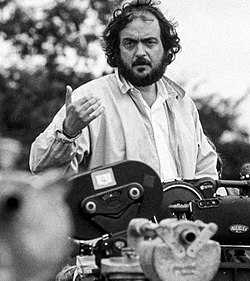
\includegraphics{kubrick}
                \caption{Stanley Kubrick (Wikipedia contributors, 2022)}
        \end{center}
\end{figure}

\FloatBarrier

\par
Stanley Kubrick might be one of the most influential filmmakers of all time. His work is admired by many cinephiles and
he is considered to be one of the most important filmmakers of the 20th century.
He is one of the main representatives of the New Hollywood Cinema and is famous for his use of long takes,
his use of natural light and the use of improvisation. He also preffered to shoot his films in real locations
and with non-professional actors which might seem familiar to you.
\\
If you ask me, when you are talking about Stanley Kubrick, you must mention his most famous close-up shooting style. According to Tony Curtis,
who is the star of Kubrick's film "Spartacus", "Kubrick had his own approach to film-making. He wanted to see the actor's faces.
He didn't want cameras always in a wide shot twenty-five feet away, he wanted close-ups, he wanted to keep the camera moving." (Wikipedia contributors, 2022)
With faces being the most important element of the films, Kubrick is very famous with the "Kubrick Stare" which is a close-up shot of the actor's
face with a forward tilt that is usually accompanied by a long take and a long pause. In his films,
he used this technique to show the inner thoughts of the characters. Generally, he used this in a dark perspective where he wanted to show
the characters are either starting to go insane or they are planning something evil.
\\

\begin{figure}[h]
        \begin{center}
                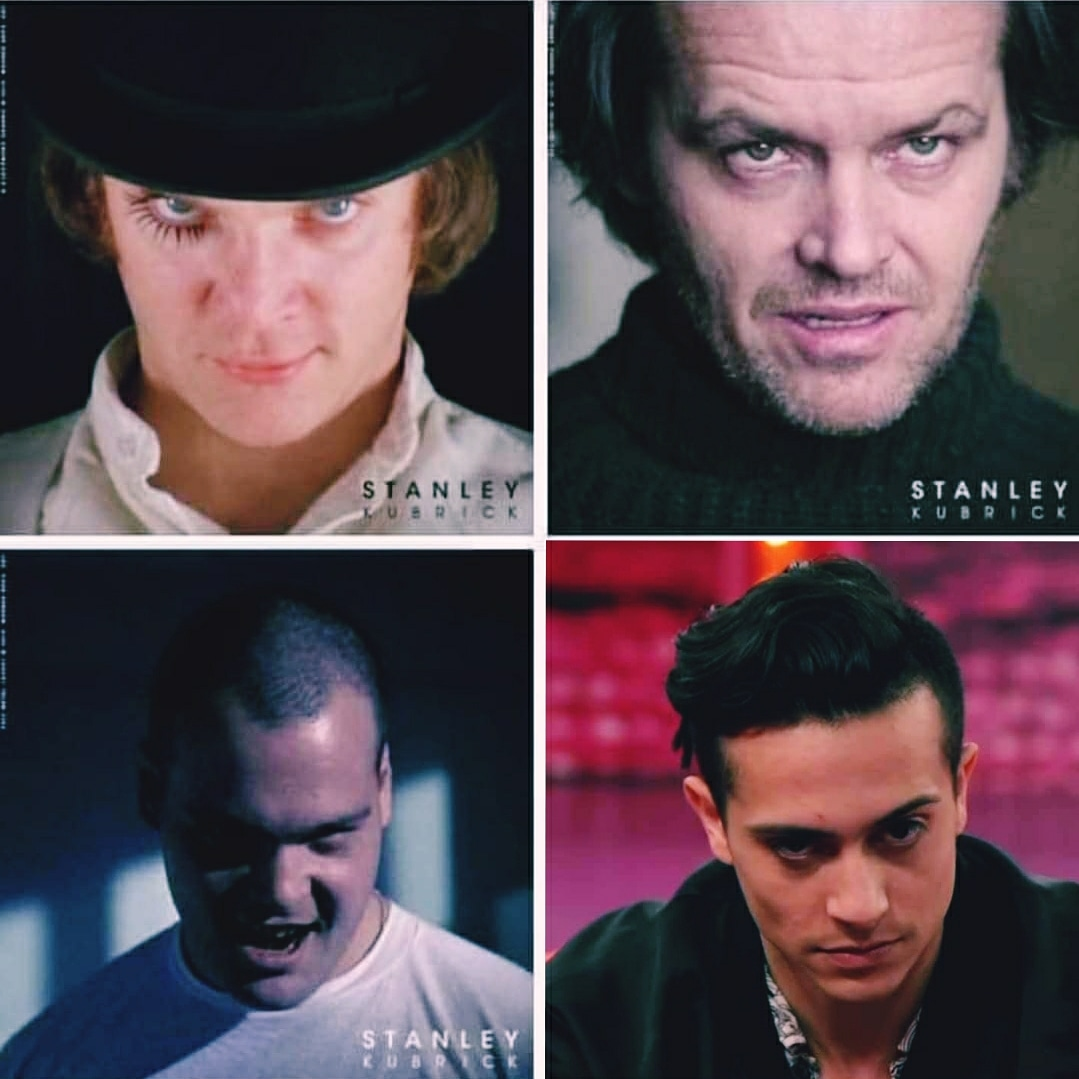
\includegraphics[width=200px]{k_stare}
                \caption{The Kubrick Stare (“the Kubrick Stare” Is One of Director Stanley Kubrick’s Most Recognizable Directorial Techniques., 2021)}
        \end{center}
\end{figure}

\FloatBarrier

\par
Now that we have talked about the French New Wave and Stanley Kubrick, let's move on to talking about the similarities between the two.
Kubrick had an authoritarian personality and he was very strict with his crew.
He liked using book plots but usually tweaked them to fit his own vision. He wanted to make the fans to fall down to his psychological games.
He also was very demanding and he was very hard to work with. He was a total perfectionist.
\\
To express on the strong authority of his, we can give the words of Shelley Duvall, who is one of the stars of Kubrick's film "The Shining".
In that movie there were several scenes that took more than 100 takes even got intothe Guinness Book of World Records
for the most retakes for a single scene with dialog. The scene where they have talked about the "shine" took 148 takes. And the more
famous and even more demanding "staircase scene" took 127 takes. And during the interview after watching the scene again with the interviewer,
Duvall stated these words about her cries and tears: "We filmed that for about 3 weeks. Every day. It was very hard. Jack was so good — so damn scary.
I can only imagine how many women go through this kind of thing." But she stated that she was also glad it was one of the best scenes in the film. (Abramovitch, 2021)
These words show how Kubrick was a very powerful author and very strict perfectionist who lived in the details,
some might also argue that these were the reasons why his movies were so successful. With his powerful mind,
he engineered his way through the movies.
\\

\begin{figure}[h]
        \begin{center}
                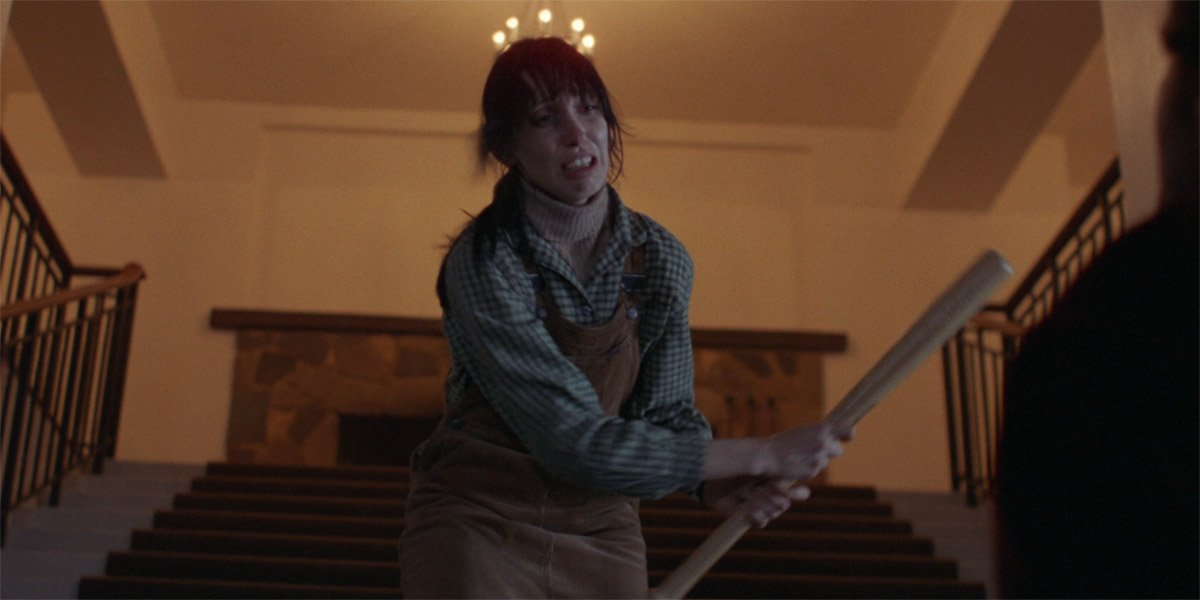
\includegraphics[width=250px]{staircase}
                \caption{The Staircase Scene (Kubrick, 1980)}
        \end{center}
\end{figure}

\FloatBarrier

\par
With a deeper dive into Kubrick's films and his words on the chronicles, we can find even more connections with the French New Wave.
Apart from him being an "Auteur" he sometimes decided to stick with the original storyline of the books too.
For example, in his film "A Clockwork Orange" he did not touch the original of the novel except for some very dark and
disturbing scenes. (Borders, 2013) In contrast, however, another connection with the French New Wave pops ups in that exact same film.
To make the film more realistic, Kubrick decided to use real locations and started searching for the right location photographs even before the production.
(Indie Film Hustle, 2020) He took his crew to the streets of London and he took them to the locations that he had found in the photographs.
This shows how New Wavevy he was. He was also very experimental and he was very open to new ideas.
\\

\begin{figure}[h]
        \begin{center}
                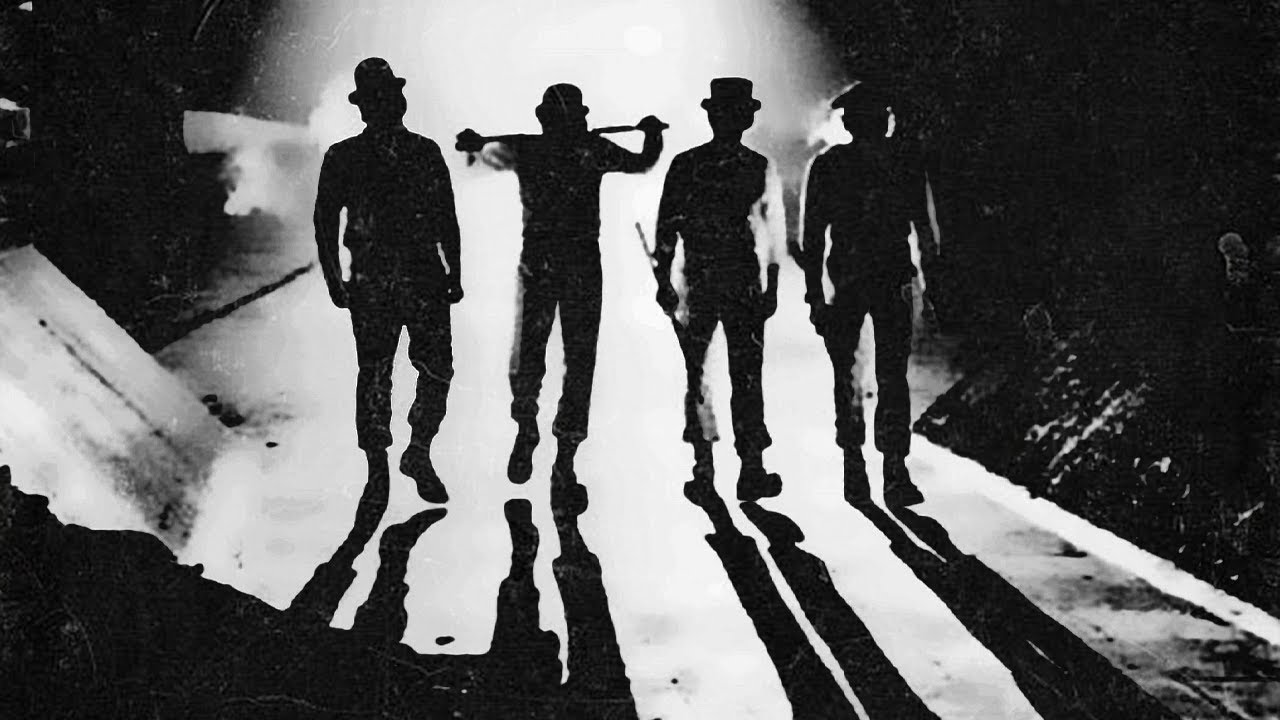
\includegraphics[width=200px]{clockorange}
                \caption{A Scene From the Streets of A Clockwork Orange (Kubrick, 1996)}
        \end{center}
\end{figure}

\FloatBarrier

\par
Apart from the similarities, Kubrick had his differences with the French New Wave too.
One major difference comes from an economical perspective, one of the key elements of the French New Wave was that it was
born out of the lack of financial resources. The filmmakers had to make their films with the limited resources that they had.
However, Kubrick had the money. In the beginning it was flowing from the Hollywood studios but later after the success of
"2001: A Space Odyssey" he earned enough money to set up a studio and finance his own films. (Wikipedia contributors, 2022)
This shows that Kubrick was a New Hollywood filmmaker who had the mindset and perspective, and also the power of a French New Wave director.
\\
From a technical perspective, Kubrick differed a bit too. Aside from the film "2001: A Space Odyssey", Kubrick did not prefer to use
too many transitions and jump-cuts. He preferred to use long takes and long pauses that were close-ups.
In addition, his perfectionism lead him to alter the scenes and not show the environment within the scenes as is.
The "Mise-en-scène" which is a French word for the design and arrangement of the scene (Wikipedia contributors, 2022) was not like French New Wave whatsoever.
Kubrick, mastered the art of the "Mise-en-scène" and he was very good at it. He was very good at creating the right and simplistic atmosphere. (StudioBinder, 2020)
This made him more than a New Hollywood and a French New Wave filmmaker.
\\

\begin{figure}[h]
        \begin{center}
                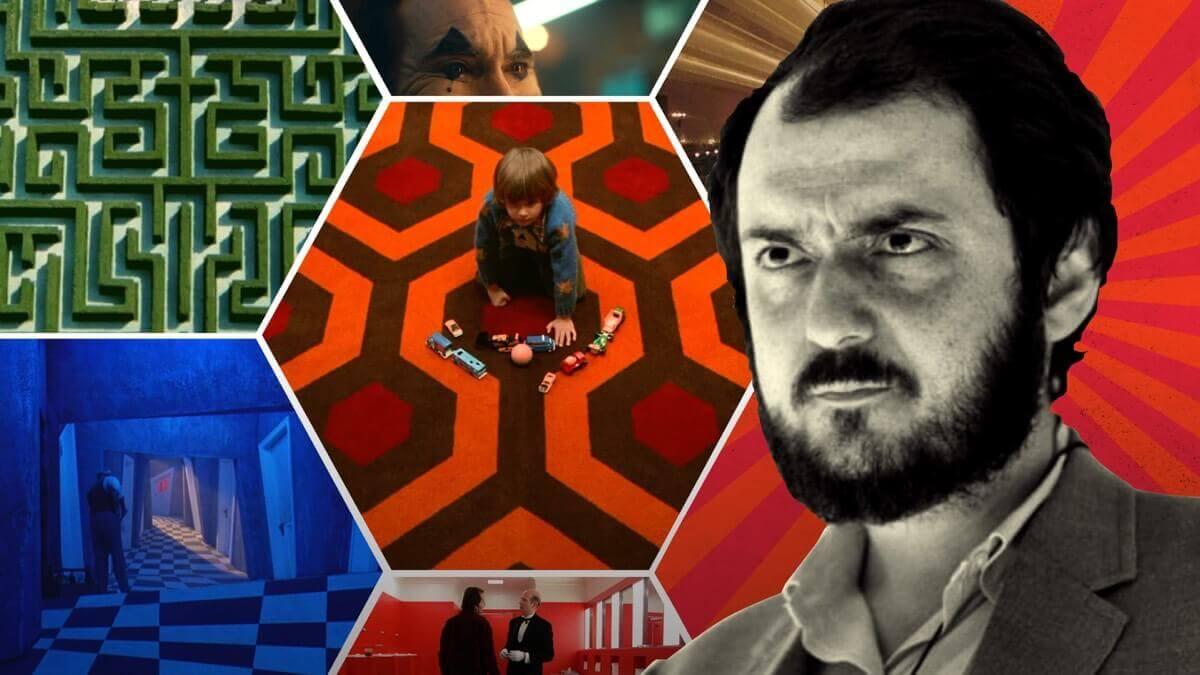
\includegraphics[width=350px]{mizansen}
                \caption{Mise-en-scène of Kubrick (StudioBinder, 2020)}
        \end{center}
\end{figure}

\FloatBarrier

\par
To sum up, Kubrick was a true "Auteur" who had a very influential and successful lifetime. As he lived in the New Hollywood era in America,
he got his roots and divergent ideas from there. But he also had the resources the french new wave directors lacked which he have gotten from the Hollywood and snowball effected from there.
He became a man of the synthesis of these two movements. He was truly a genius and a master of his craft. As he knew that, he used the auteurial power to assert his dominance over the films
and mark them as his own. And even though he was criticisized by many writers like Stephen King who said Kubrick's adaptation was the only one he can remember hating,
(Borders, 2013) it seems like he knew what he was doing. As he was one of the filmmakers who got famous when he was still alive and
being produced the most famous and influential films of all time, according to some of us cinephiles of course.
\\

% Bibliography
\section*{Bibliography}
% numbered list
\begin{enumerate}
        \item The Editors of Encyclopaedia Britannica. (2017, December 27). auteur theory | Definition and Directors. Encyclopedia Britannica. \url{https://www.britannica.com/art/auteur-theory}
        \item Wikipedia contributors. (2022, October 24). Stanley Kubrick. Wikipedia. \url{https://en.wikipedia.org/wiki/Stanley_Kubrick}
        \item “The Kubrick Stare” is one of director Stanley Kubrick's most recognizable directorial techniques. A method of shot composition where a character stares at the camera with a forward tilt, to convey to the audience that they are at the peak of their derangement. (2021, February 16). Reddit. \url{https://www.reddit.com/r/rupaulsdragrace/comments/lleo4l/the_kubrick_stare_is_one_of_director_stanley/}
        \item Abramovitch, S. A. (2021, February 11). Searching for Shelley Duvall: The Reclusive Icon on Fleeing Hollywood and the Scars of Making ‘The Shining.’ The Hollywood Reporter. https://www.hollywoodreporter.com/feature/searching-for-shelley-duvall-the-reclusive-icon-on-fleeing-hollywood-and-the-scars-of-making-the-shining-4130256/
        \item Borders, M.B. Book vs. Film: A Clockwork Orange. (n.d.). LitReactor. Retrieved October 31, 2022, from \url{https://litreactor.com/columns/book-vs-film-a-clockwork-orange}
        \item Kubrick, S. K. (Director). (1980, May 23). The Shining (Original).
        \item Indie Film Hustle. (2020, June 9). Stanley Kubrick: A Clockwork Orange - The Directors Series [Video]. YouTube. \url{https://www.youtube.com/watch?v=aCDsB4bmDAE}
        \item Kubrick, S. K. (Director). (1996, March 15). A Clockwork Orange (Original).
        \item StudioBinder. (2020, September 13). What is Mise en Scène in Film: Definition and Examples. \url{https://www.studiobinder.com/blog/mise-en-scene/}
\end{enumerate}

\end{document}